
% Template for Elsevier CRC journal article
% version 1.1 dated 16 March 2010

% This file (c) 2010 Elsevier Ltd.  Modifications may be freely made,
% provided the edited file is saved under a different name

% This file contains modifications for Procedia Computer Science
% but may easily be adapted to other journals

% Changes since version 1.0
% - elsarticle class option changed from 1p to 3p (to better reflect CRC layout)

%-----------------------------------------------------------------------------------

%% This template uses the elsarticle.cls document class and the extension package ecrc.sty
%% For full documentation on usage of elsarticle.cls, consult the documentation "elsdoc.pdf"
%% Further resources available at http://www.elsevier.com/latex

%-----------------------------------------------------------------------------------

%%%%%%%%%%%%%%%%%%%%%%%%%%%%%%%%%%%%%%%%%%%%%%
%%%%%%%%%%%%%%%%%%%%%%%%%%%%%%%%%%%%%%%%%%%%%%
%%                                          %%
%% Important note on usage                  %%
%% -----------------------                  %%
%% This file must be compiled with PDFLaTeX %%
%% Using standard LaTeX will not work!      %%
%%                                          %%
%%%%%%%%%%%%%%%%%%%%%%%%%%%%%%%%%%%%%%%%%%%%%%
%%%%%%%%%%%%%%%%%%%%%%%%%%%%%%%%%%%%%%%%%%%%%%

%% The '3p' and 'times' class options of elsarticle are used for Elsevier CRC
% \documentclass[review]{elsarticle}
\documentclass[times]{elsarticle}


%% Give the name of the journal
\journal{Journal of Computational Science}


%% The amssymb package provides various useful mathematical symbols
\usepackage{amssymb}
\usepackage{amsmath}


 

% Path to the figures
\graphicspath{{figures/}}

% if you have landscape tables
% \usepackage[figuresright]{rotating}
\usepackage{color}



% Mathetmatical symbols
\newcommand{\tr}{\mathrm{tr} \hspace{0.05cm} }
\newcommand{\argmax}{\mathrm{argmax} \hspace{0.05cm} }

% End-systolic elastance
% \newcommand{\Es{E_{\text{ES}}}}
% \newcommand{\es}{_{\max}}
\newcommand{\es}{_{\text{ES}}} 

% Mechanics
\newcommand{\Xvec}{\mathbf{X}}
\newcommand{\xvec}{\mathbf{x}}
\newcommand{\uvec}{\mathbf{u}}
\newcommand{\N}{\mathbf{N}}
\newcommand{\plv}{p_{\textnormal{\tiny{lv}}}}

% Functionals
\newcommand{\Istrainavg}{\overline{I}_{\text{strain}}}
\newcommand{\Istrainrelmax}{\overline{I}^{\text{relmax}}_{\text{strain}}}
\newcommand{\Ivolavg}{\overline{I}_{\text{vol}}}

% Fiber -sheets
\newcommand{\ef}{\mathbf{f}_0}
% \newcommand{\es}{\mathbf{s}_0}
% \newcommand{\en}{\mathbf{e}_n}
\newcommand{\Fef}{\mathbf{f}}

% Local basis
\newcommand{\ec}{\mathbf{e}_c}
\newcommand{\V}[1]{\bm{#1}}

% Tensors
\newcommand{\C}{\mathbf{C}}
\newcommand{\F}{\mathbf{F}}
\newcommand{\I}{\mathbf{I}}
\newcommand{\T}{\mathbf{T}}
\newcommand{\B}{\mathbf{B}}

% Stress tensors
\newcommand{\FPiola}{\mathbf{P}}
\newcommand{\SPiola}{\mathbf{S}}
\newcommand{\Cauchy}{\mathbf{\sigma}}


\begin{document}

\begin{frontmatter}

\title{Estimating cardiac contraction through high resolution data
  assimilation of a personalized mechanical model}


\author[simula,uioinf,cci]{Henrik Finsberg\corref{cor1}\fnref{label1}}
\ead{henriknf@simula.no}
\author[kcl]{Gabriel Balaban}
\author[uiomed,cci]{Hans Henrik Odland}
\author[uiomed,cci]{Stian Ross}
\author[simula,uioinf,cci]{Joakim Sundnes}
\author[simula,aas,cci]{Samuel Wall}

\address[simula]{Simula Research Laboratory, P.O. Box 134 1325
  Lysaker, Norway}
\address[uioinf]{Department of Informatics, University of Oslo,
  P.O. Box 1080, Blindern 0316 Oslo, Norway}
\address[uiomed]{Faculty of Medicine, University of Oslo, P.O. Box
  1078 Blindern, 0316 Oslo, Norway}
\address[cci]{Center for Cardiological Innovation, Songsvannsveien 9,
  0372 Oslo, Norway}
\address[aas]{Department of Mathematical Science and Technology,
  Norwegian University of Life Sciences,  Universitetstunet 3 1430 Ås,
  Norway}
\address[kcl]{Department of Imaging Sciences and Bioengineering,
              King's College London, St. Thomas Hospital, 
              Westminster Bridge Rd, Lambeth, London SE1 7EH, UK}
            
\cortext[cor1]{Corresponding author}

 
  
\begin{abstract}
  
Cardiac computational models, individually personalized, can provide
clinicians with useful diagnostic information and aid in
treatment planning.  A major bottleneck in this process can be  
determining model parameters to fit created models to individual
patient data. However, adjoint-based data assimilation techniques can
now rapidly estimate high dimensional parameter sets.  This method is
used on a cohort of heart failure patients, capturing cardiac mechanical
information and comparing it with a healthy control group.  Excellent
fit ($R^2 \geq 0.98$) to systolic strains is obtained, and analysis
shows a significant difference in estimated contractility between the
two groups.

\end{abstract}

\begin{keyword}
%% keywords here, in the form: keyword \sep keyword

%% MSC codes here, in the form: \MSC code \sep code
%% or \MSC[2008] code \sep code (2000 is the default)
Cardiac Mechanics \sep Adjoint Method \sep Data assimilation \sep
PDE-constrained optimization \sep Contractility 
\end{keyword}

\end{frontmatter}

% \pagebreak
%%
%% Start line numbering here if you want

% \linenumbers

%% main text
\section{Introduction}
\label{sec:introduction}

Patient-specific cardiac modeling has emerged as a potential tool
for clinical diagnosis as well as treatment
 optimization\cite{viceconti2016virtual}.  By linking
patient measurements to physical processes through a mathematical
framework, models can provide us with additional insight into
cardiac function or dysfunction at the level of the
individual. However, the complexity of the heart makes this difficult,
and this is recognized as a key challenge in modern bioengineering
\cite{hunter2010vision}. 

One difficulty is the effort to personalize models and
simulations to individual patients.  While a wealth of clinical 
data exists to parameterize such 'patient-specific' models, methods to
assimilate this data into simulations can involve extensive
computation time, often putting them outside the scope of clinical
utility. However, new methods are emerging to improve the flow of clinical
measurements into powerful data driven simulations.  Automated
geometry segmentation \cite{rabben2010technical} and improved
optimization techniques \cite{chabiniok2012estimation}, can improve the
speed at which patient-specific models can be built and parameterized.
In particular, recent advancements in adjoint-based data assimilation
techniques \cite{balaban} offer an efficient way to assimilate ventricular mechanical
 information using highly spatially resolved parameters.  
 
Here we use an adjoint based assimilation
method with a mechanical model in order to construct simulations that
accurately reflect clinical motion data, both for
healthy controls and patients suffering from left bundle
branch block (LBBB). The use of a highly spatially resolved 
contraction parameter, enabled through adjoint-methods, provides excellent data fit to
measured strains and volumes, and fit models provide estimates of cardiac
contraction.   Such biomarkers may prove useful to
clinicians for diagnoses of problems with cardiac function, and to
better plan therapies.    

\section{Materials and methods}
\label{sec:methods}

\subsection{Data acquisition}
\label{sec:clinical_data}

Clinical measurements of cardiac function for seven LBBB patients were
obtained from the Impact study \cite{ImpactStudy2016}.
Data was also acquired for seven healthy volunteers. 4D echocardiographic
images of the left ventricle (LV), for both the LBBB patients and
healthy subjects, were captured using
a GE Vingmed E9 device, and analysis carried out with the
software package EchoPac. For each subject, depending on frame rate and cardiac cycle time, the
analysis provided between 15 and 50 LV volumes,  geometric segmentations of the LV
endocardium and epicardium, and cardiac strain calculated via speckle
tracking. The strains were defined according to
the 17 segment AHA-zone representation
\cite{cerqueira2002standardized}, in the longitudinal, radial and
circumferential direction, giving a total of 51 strain measurements
per time point.

The LBBB patients had LV pressure measurements taken during
implantation of a cardiac resynchronization therapy (CRT) device, and
valvular events were used to synchronize the pressure to the echo data
with the help of a medical doctor.  Meanwhile, in the 
healthy control group, where invasive pressure measurements were
absent, the pressure waveform from one of the LBBB patients was used and
scaled to reported values of the end-diastolic and end-systolic
left ventricular pressure [Table 30-1 in \cite{klingensmith2008washington}].


\subsection{Automated geometry and microstructure creation}
For each patient, a 3D tetrahedral mesh of the LV was
constructed using Gmsh \cite{geuzaine2009gmsh} from triangulated
segmented surfaces of the endo- and epicardium at the beginning of
atrial systole, Figure \ref{fig:pipeline}. A cut was made at the
ventricular base of the segmentation, so that the mesh cavity volume
and the ultrasound measured volume differed by less than  $1$ ml. Mesh
cells were marked into the 17 AHA regions through the regionally
delineated strain data, and the myocardial fiber orientation were
assigned using the algorithm from Bayer et al \cite{bayer2012novel},
with the endo- and epicardial helix fiber angles set to
$\alpha_{\text{endo}} = 60$ and $\alpha_{\text{epi}} = -60$, respectively.

\subsection{Mechanical Model}
We represent the heart as a hyperelastic continuum body, where the coordinates in
the reference($\Xvec$) and the current($\xvec$) configuration are
related via the displacement field $\uvec = \xvec-\Xvec$. Furthermore,
we utilize the
deformation gradient, the determinant of the deformation gradient
and, the right Cauchy-Green deformation tensor given by $\F= \I+\nabla
\uvec $,  $J = \det \F$ and $\C = \F^T\F$, respectively. 
% Constitutive relations
To model the passive behavior of the myocardium, the transversely 
isotropic strain energy function proposed in  \cite{holzapfel2009constitutive} is adopted:
\begin{align}
\label{eq:hoa}
  \mathcal{W}(I_1, I_{4\ef}) = \frac{a}{2 b} \left( e^{ b (I_1 
  - 3)}  -1 \right)
  + \frac{a_f}{2 b_f} \left( e^{ b_f (I_{4\ef} 
  - 1)_+^2} -1 \right).
\end{align}
Here $I_1 = \tr \C$ and $I_{4\ef}= \ef \cdot (\C \ef)$ are invariants
of $\C$, $(\cdotp)_{+}  = \max\{\cdot, 0\}$, and $a, a_f, b, b_f$ are
material stiffness parameters defining the elastic properties of the myocardium.
% Incompressibility
We follow a common approach and assume that the myocardium is incompressible. 
Incompressibility is incorporated in the model by using a two-field variational 
approach, where we introduce a Lagrange multiplier $p$ which represents the 
hydrostatic pressure, and the term $p(J-1)$ is added to the strain-energy.
% Active response
To model the active response we apply the active strain framework
\cite{ambrosi2011electromechanical}, decomposing the deformation into
elastic and active components, $\F = \F_e \F_a$. The active part,
$\F_a$ represents the actual shortening along the muscle fibers, while
the elastic part $\F_e$ ensures compatibility of the tissue. We adopt
the formulation of the active deformation gradient from
\cite{gjerald2014patient}, with the following form:  
\begin{equation}
  \F_a =
  (1 - \gamma) \ef \otimes \ef
  + \frac{1}{\sqrt{1 - \gamma}} (\I - \ef \otimes \ef).
 \label{eq:active_strain_Fa_gjerald}
\end{equation}
%which accounts for the effect of shortening along muscle fibers \cite{gjerald2014patient},
%while the elastic part $\F_e$ captures the elastic deformation of the tissue. 
In this formulation of $\F_a$, $\gamma$ prescribes the relative active shortening
along the fibers, and is implemented as a piecewise linear function over
the domain, yielding one parameter per vertex in the mesh. The active
model is coupled to the passive model by letting
$\mathcal{W}$ in \eqref{eq:hoa} be a function of the
modified elastic invariants $I_1^E = \tr \C_e$ and $I_{4\ef}^E = \ef
\cdot (\C_e \ef)$, where $\C_e = \F_e^T\F_e$.

The resulting displacement field $\uvec$ and hydrostatic pressure $p$
are determined by using the principle of stationary potential energy
\cite{holzapfel2000nonlinear}, which is based on minimizing the total
energy  $\Pi(\uvec, p)$, which includes internal energy derived from
\eqref{eq:hoa} and external energy. The external energy includes
contributions from the measured cavity pressure $p_{\text{LV}}$, and a
linear spring term at the basal boundary, with spring constant
$k$ = 1 kPa. The equilibrium solution is found by solving for the minimum
potential energy, $\delta\Pi(\uvec, p) = 0$. 

\subsection{Data Assimilation}
In order to constrain the model to each patient's clinical measurements, we
consider a PDE-constrained optimization problem where
the objective functional is given by the misfit between
simulated and measured strain and volume along with a first order Tikhonov regularization of the
model parameters.
\begin{equation}
  \begin{aligned}
    \label{eq:pde_opt}
    & \underset{m}{\text{minimize}}
    & &  \alpha \left( \frac{V^i - \tilde{V}^i}{V^i} \right)^2
    + (1-\alpha)  \sum_{j= 1}^{17} \sum_{k \in \{c,r,l\}}  \left( \varepsilon_{kj}^i
      -  \tilde{\varepsilon}_{kj}^i \right)^2
    + \lambda \| \nabla m^i \|^2 \\
    & \text{subject to}
    & & \delta \Pi(\uvec, p) = 0.
  \end{aligned}
\end{equation}


Here $V$ and $\varepsilon_{kj}$ are the measured volume and regional Lagrangian strain in
segment $j$ in direction $k$ respectively, and $\tilde{V}^i =
-\frac{1}{3} \int_{\partial \Omega_{\text{endo}}} (\Xvec + \uvec)
\cdotp J\F^{-T}\N  \mathrm{d}S$,  and $\varepsilon_{kj} =
\frac{1}{|\Omega_j|}\int_{\Omega_j}  \mathbf{e}_k^T \nabla \uvec \,
\mathbf{e}_k  \mathrm{d}x.$ 
The parameters $\alpha$ and $\lambda$
control the weights on the different terms, and the sum in the second
term is taken over the seventeen AHA
segments, and the three different strain components (Section \ref{sec:clinical_data}).


The data assimilation procedure is divided into two phases; a passive
phase and an active phase. For the passive phase we find the stiffness
of the overall ventricle,  using the control parameter $m = a$, where
$a$ is the linear isotropic parameter in \eqref{eq:hoa}, $\alpha=
1.0$,  with $\lambda = 0$ and $\gamma = 0$, minimizing only the misfit
with the measured volumes. The remaining material parameters are fixed
according to [Table 1 row 3 of \cite{holzapfel2009constitutive}].
For the active phase we fix the material
parameter optimized in the passive phase, and the control parameter
becomes the pointwise relative mechanical contraction, $m = \gamma$,
with $\alpha = 0.95$ and $\lambda = 0.01$. This choice of $\alpha$ and
$\lambda$ was based on the analysis done in \cite{balaban}. A summary
of our optimization pipeline is provided to the right in
Figure~\ref{fig:pipeline}.  

\begin{figure}[htbp]
\centering
    \includegraphics[width=\textwidth]{models}
\caption{Left: Automated anatomical modeling pipeline to produce AHA
  marked simulation meshes with applied fiber orientations from 3D
  echocardiographic segmentations. Right: Optimization
  pipeline. 1. Optimization of passive model is
  initialized. 2. Linear isotropic material parameter
  $a$ in \eqref{eq:hoa} as control parameter, minimize the misfit
  between simulated and measured volume from beginning of atrial
  systole to end diastole. 3. Fix the optimized value of $a$, let
  $\gamma$ from \eqref{eq:active_strain_Fa_gjerald} be zero,
  and initialize the active model. 4. Using $\gamma$ from
  the previous point as initial guess, minimize the misfit between
  volume and regional strain using $\gamma$ as control. Continue until
  all points in the cardiac cycle are optimized.}
\label{fig:pipeline}
\end{figure}

\subsection{Finite element solution}
We employ a Galerkin finite element method with Taylor-Hood
tetrahedral elements, that is $(\uvec, p) \in \mathbb{P}_2 \times
\mathbb{P}_1 $, with $\mathbb{P}_n$ being the space of piecewise
polynomials of degree $n$.
The solver is implemented in the finite element framework FEniCS
\cite{logg2012automated}, and uses a Newton trust region algorithm
\cite{PETScPackage} to solve nonlinear systems. The minimization of the
model-data misfit functional~\eqref{eq:pde_opt} is accomplished by a sequential
quadratic programming algorithm (SQP)~\cite{kraft1988software}, where
the functional gradient is computed by solving an automatically derived adjoint
equation \cite{farrell2013automated}. In these minimizations an upper bound of $0.4$ is
set for the control variable $\gamma$.

\subsection{Contraction analysis}
The optimized spatially resolved contraction parameter $\gamma$ from 
\eqref{eq:active_strain_Fa_gjerald}, may be interpreted as an
index of contractility, as it describes how much the material attempts
to contract independent of elastic load.  Since this parameter is
defined at all the nodal points in the geometry, we summarize the
contraction of the LV by averaging over the entire ventricular 
domain, $ \overline{\gamma}(t) = \frac{1}{|\Omega|} \int_{\Omega}
\gamma (t, \mathbf{x}) \mathrm{d}\mathbf{x}$, at each time point 
to provide a trajectory of average ventricular contraction for
each patient. In addition, the overall elastic state of the optimized patient models
can be used to give estimates of LV elastance. The left ventricular
end-systolic elastance $E\es$, the response of end systolic volume to
increased load, is considered to be one of the major determinants for
cardiac systolic function, and was in \cite{sagawa1977end} proposed
as a global index of ventricular contractility. 
It is possible to calculate the end systolic elastance directly 
if the end systolic pressure is known or estimated, 
by perturbing the loading conditions on the optimized model at end
systole, and calculating the slope in the resulting
ES pressure-volume curve. More precisely, if $\plv^{\text{ES}}$ is the
end-systolic ventricular pressure, with cavity volume $V^{\text{ES}}$,
we change the pressure to $\plv^{\text{ES} + \Delta} =
\plv^{\text{ES}} + \Delta \plv$, resulting in a change in volume,
$V^{\text{ES} +\Delta} = V^{\text{ES}} + \Delta V$. The end-systolic
elastance can then be estimated by 
\begin{align}
  \tilde{E}\es = \frac{\Delta \plv}{\Delta V}.
  \label{eq:estimate_elastance}
\end{align}

\section{Results and discussion}
\label{sec:results}


\subsection{Matching of strain and volume}
We show the results from two representative simulations in
Figure~\ref{fig:generic_result}, one from the LBBB group and one from
the healthy control group. Snapshots from the calculated end-diastolic and
end-systolic configurations are depicted, and agreement with PV-loops
and one of the 51 strain traces over the cardiac cycle shown.  


\begin{figure}[htbp]
  \centering
  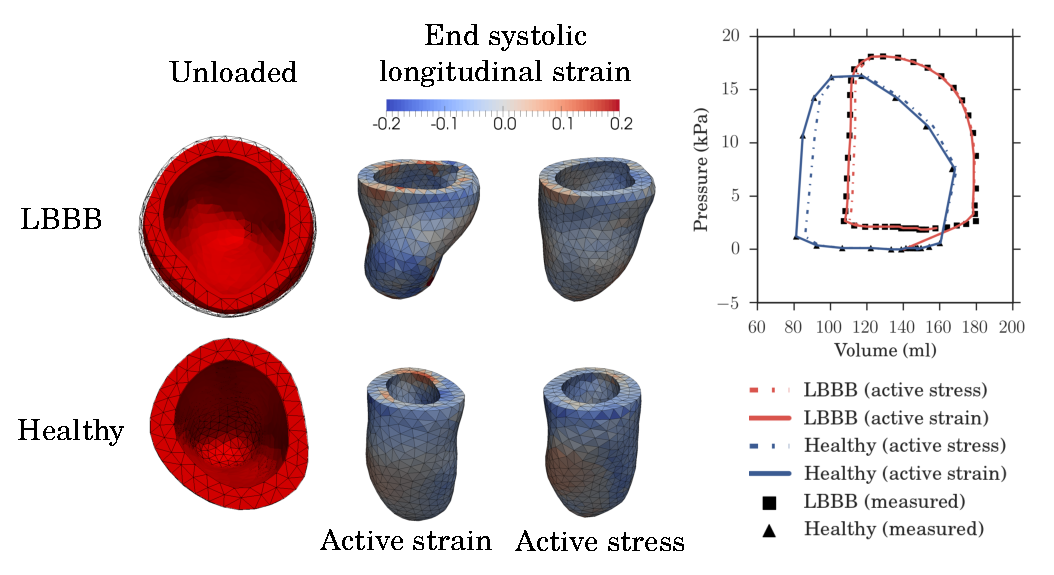
\includegraphics[width=\textwidth]{generic_result}
  \caption{Left: Snap shots of end-diastolic(ED) and end-systolic(ES)
    model configurations for an LBBB patient and a healthy
    control. The colormaps shows longitudinal strain. Right: Simulated
    and measured or estimated pressure-volume loops for these hearts,
    as well as the longitudinal strain traces for both in the mid
    septal segment, one of the 51 strain traces optimized. This mid
    septal segment is highlighted in green in the left figure.}
  \label{fig:generic_result}
\end{figure}


The total analysis of the 14 patients involved optimizing 432 volume
measurements and 20 853 strain measurements. The average time for one
forward and gradient evaluation was 8.3 and 8.9 seconds respectively
when running on a cluster using four cores. Here the average number of
control parameters was 985.

In order to visualize the overall match of simulated to measured data,
we show linear regression plots in Figure~\ref{fig:data_matching}. For
the strain, we separately consider the diastolic and systolic points,
as different types of data were used to  constrain the model in these
two phases, namely volume in the diastolic phase and strain in the
systolic phase. An excellent overall fit was obtained for the optimized
volume ($R^2=1.00$) and systolic strains ($R^2=0.98$). 
Diastolic strains, not used in the optimization, were less well
matched ($R^2=0.29$). 

\begin{figure}[htbp]
  \centering
  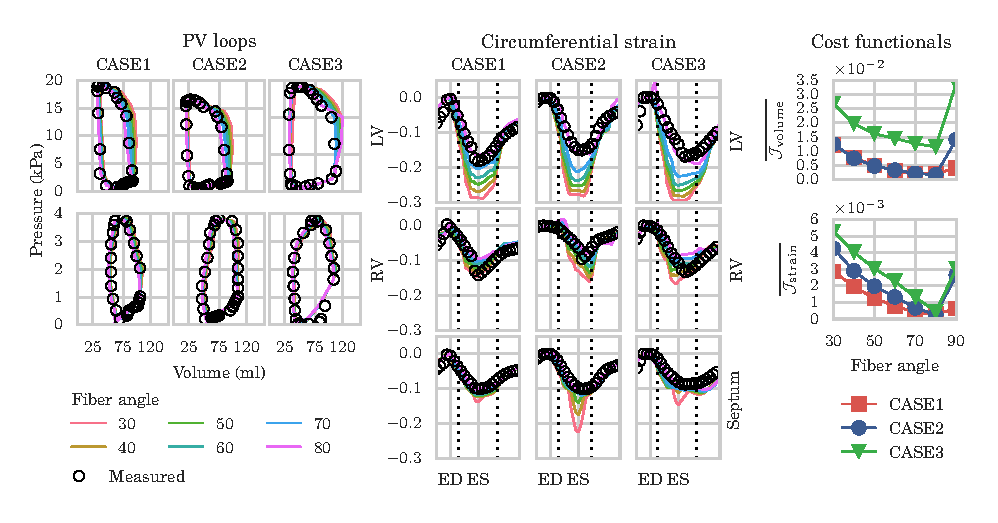
\includegraphics[width=\textwidth]{data_matching}
  \caption{Left: Scatter plot of simulated versus
    measured volumes and the best linear least-squares fit of these
    points, (slope = 1.00). Right: Scatter plot of simulated versus
    measured strain for all segments and all directions, separated
    into the diastole, were only the volume was optimized and systole,
    where both the strain and volume were optimized. The best linear
    least-squares fit for the two cases. For diastole, the slope of
    the best linear fit was $0.35$, while the linear fit for the
    systolic points had a slope of $0.98$.}
  \label{fig:data_matching}
\end{figure}


\subsection{Estimation of global contractility and elastance}

Global contraction time courses, $\overline{\gamma}$, for each 
patient were synchronized to the valvular
events to normalize for differing cycle lengths. The average 
and standard deviation of these normalized traces for the
LBBB vs the healthy controls are shown in right of
Figure~\ref{fig:contractility}. The healthy patients had a much higher
level of contraction through the cardiac cycle, and the peak values
were compared using one-way ANOVA, yielding a $P-$value less than
$0.001$. 

The values of calculated $\tilde{E}\es$ for the healthy and LBBB patients are
shown to the left in Figure~\ref{fig:contractility}. The calculated
elastances of the LBBB group were significantly lower than for the healthy
group, with the comparison between the groups using one-way ANOVA
giving a $P-$value of $0.047$. 




\begin{figure}[htbp]
  \centering
  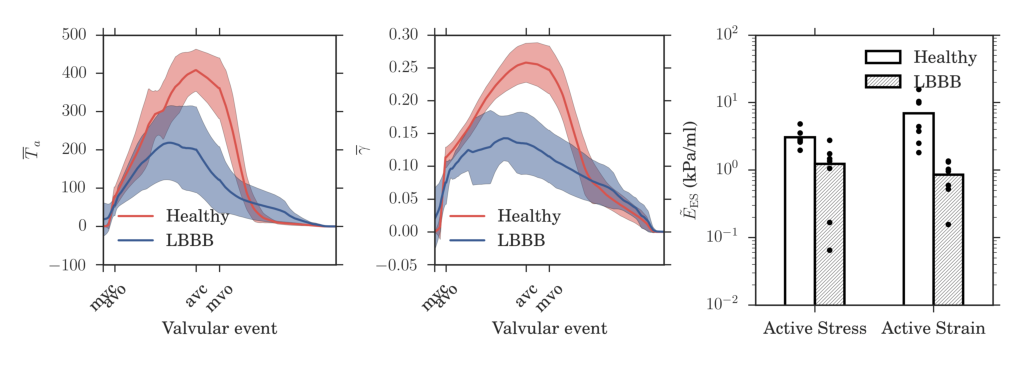
\includegraphics[width=\textwidth]{contractility}
  \caption{Left: Estimated values of $\tilde{E}\es$, given by
    \eqref{eq:estimate_elastance}. The mean value is depicted for each
    group as a bar. Right: Mean value of $\gamma$ for the two groups
    synchronized with respect to valvular events (mvc: mitrial valve
    closure, avo: aortic valve opening, avc: aortic valve closure,
    mvo: mitrial valve opening). Shaded area represents $\pm 1$
    standard deviation.} 
  \label{fig:contractility}
\end{figure}



\section{Discussion}
In this study we applied an adjoint-based data assimilation technique
to constrain patient data to a cardiac mechanics model.
LV pressure was used as a boundary condition, while LV
volume and regional strain were assimilated by the means of a
spatially varying contraction parameter. We tested this methodology on a group of
seven healthy control patients and seven patients
diagnosed with LBBB. The results gave an excellent fit between the measured
and simulated volume and systolic strain ($R^2 \geq 1.00$ and $R^2
\geq 0.98$, respectively) for more than 21,000 observation points.
Diastolic strains, which were not included in the optimization, had a
much poorer fit, demonstrating the need for consideration of regional
variations in order to create models that can accurately fit patient
data.   

These calibrated models allow us to quantify aspects of cardiac
contractility.   We estimated the traditional measure of end-systolic
elastance, by perturbations of the model at the end systolic
configuration.  The healthy control group had significantly higher
end-systolic elastance than the LBBB group, although limitations exist
with these calculations due to using a synthetic pressure curve with
the healthy group.  However, the values calculated by using direct
pressure readings for the LBBB group (3 - 10 mmHg) are slightly higher
but correspond very well with the range provided for a heart failure
cohort of (0.5 - 4.9 mm Hg) \cite{senzaki1996single}.  Along with the
end-systolic elastance estimates, our simulations also were use to
compare the average value of $\gamma$, which may also be interpreted
as an index on contractility, between the two groups through the
cardiac cycle. Again, the healthy controls showed a significantly
higher peak value, compared to the LBBB group. The relationship
between $\gamma$ and $\tilde{E}\es$ remains to be investigated.


\section{Conclusions}

Adjoint-based data assimilation are a powerful technique for
estimating high dimensional parameters in order to incorporate large
amounts of information into a model. Although limitations in our
patient data and assumptions remain, we have demonstrated how such
techniques can be applied to problems in mechanics for use in
estimating indices of cardiac contractility.   Future work will be
used to adjust and improve such models and work towards their
validation and clinical utility.   

 %It should be
%stressed that the need to for validation is a necessary next step, to
%further adjust and improve such models.

\section*{Acknowledgments}
This study was funded by Research Council of Norway: Center for
Biomedical Computing at Simula Research Laboratory and Center for
Cardiological Innovation at Oslo University Hospital.
%, grant number 179578 and 203489.
Computations were performed on the Abel supercomputing cluster at the 
University of Oslo via a Notur project.
% project nn9249k.


%% References
%%
%% Following citation commands can be used in the body text:
%% Usage of \cite is as follows:
%%   \cite{key}         ==>>  [#]
%%   \cite[chap. 2]{key} ==>> [#, chap. 2]
%%

%% References with BibTeX database:
% \pagebreak
\bibliographystyle{elsarticle-num}
\bibliography{bibliography}
%% Authors are advised to use a BibTeX database file for their reference list.
%% The provided style file elsarticle-num.bst formats references in the required Procedia style

%% For references without a BibTeX database:

% \begin{thebibliography}{00}

%% \bibitem must have the following form:
%%   \bibitem{key}...
%%

% \bibitem{}

% \end{thebibliography}

\end{document}

%%
%% End of file `ecrc-template.tex'. 